\documentclass[11pt,a4paper]{article}
\usepackage[utf8]{inputenc}
\usepackage[T1]{fontenc}
\usepackage[margin=1in]{geometry}
\usepackage{xcolor}
\usepackage{tcolorbox}
\usepackage{booktabs}
\usepackage{pgfplots}
\pgfplotsset{compat=1.18}
\usepackage{sectsty}

\usepackage{mathpazo} % nice font

% Define colors
\definecolor{brandblue}{HTML}{0D47A1}
\definecolor{goodgreen}{HTML}{2E7D32}
\definecolor{badred}{HTML}{C62828}
\definecolor{surface}{HTML}{F8F9FA}

\sectionfont{\color{brandblue}}

\begin{document}

\begin{center}
{\Huge\bfseries\color{brandblue} Trading Performance Analytics}\\[0.5em]
{\Large Executive Summary Report}\\[1em]
{\large Prepared for \textbf{Mission Credit Card}}\\[0.5em]
{\small Generated on \today}
\end{center}
\vspace{1em}

% Headline stats
\begin{tcolorbox}[colframe=brandblue, colback=surface, title=Free Tier --- Trade Log Transparency, title filled=true, fonttitle=\bfseries\large]
\begin{center}
\renewcommand{\arraystretch}{1.5}
\begin{tabular}{p{0.3\textwidth} p{0.3\textwidth} p{0.3\textwidth}}
\textbf{Total Net P\&L} & \textbf{Win Rate} & \textbf{Profit Factor} \\
{\Large \color{badred} \$-715.16} & {\Large 25.0\%} & {\Large 0.66} \\
\end{tabular}
\end{center}
\vspace{0.5em}
\hrule
\vspace{0.5em}
\begin{center}
\renewcommand{\arraystretch}{1.2}
\begin{tabular}{cccc}
\textbf{Total Trades:} & 28 & & \\
\textbf{Average Win:} & \color{goodgreen} \$202.67 & \textbf{Average Loss:} & \color{badred} \$-101.61 \\
\end{tabular}
\end{center}
\end{tcolorbox}

\vspace{1.5em}
\begin{tcolorbox}[colframe=brandblue, colback=white, title=Explainability \& Core Insights, fonttitle=\bfseries]
\begin{itemize}
\setlength\itemsep{0.3em}
\item Your most profitable direction is \textbf{Buy} netting \$17.84. Consider focusing your specific setups here.
\item Longer duration trades ($\geq$ 5 min) outearned scalps (\$-49.72 vs \$-665.44). Let winners run.
\end{itemize}
\end{tcolorbox}

\vspace{1.5em}
\begin{tcolorbox}[colframe=goodgreen!80!black, colback=white, title=Suggested Improvements, fonttitle=\bfseries]
\begin{itemize}
\setlength\itemsep{0.3em}
\item Net P\&L is negative. Consider cutting your sizing down to 1 contract exclusively until consistency improves.
\item With a 25.0\% win rate, try reducing trade frequency and only taking A+ setups. Patience will naturally lift this metric.
\end{itemize}
\end{tcolorbox}

\vspace{1.5em}
\subsection*{Directional Split}
\begin{center}
\renewcommand{\arraystretch}{1.2}
\begin{tabular}{@{} l r r r r @{}}
\toprule
\textbf{Direction} & \textbf{Trades} & \textbf{Win Rate} & \textbf{Profit Factor} & \textbf{Net P\&L} \\
\midrule
\textbf{Buy} & 11 & 27.3\% & 1.02 & \color{goodgreen} \$17.84 \\
\textbf{Sell} & 17 & 23.5\% & 0.44 & \color{badred} \$-733.00 \\
\bottomrule
\end{tabular}
\end{center}

\vspace{1em}
\subsection*{Equity Curve}
\begin{center}
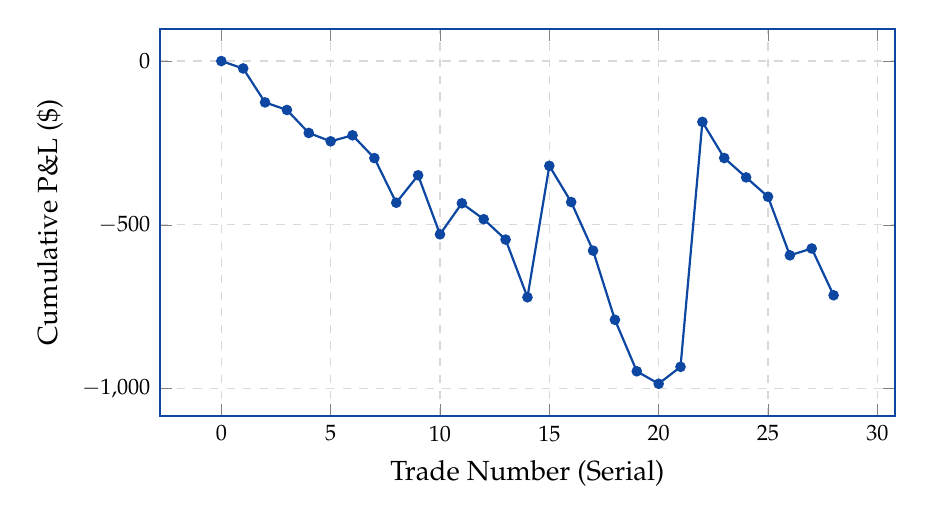
\begin{tikzpicture}
\begin{axis}[
    width=0.9\textwidth,
    height=6.5cm,
    grid=major,
    grid style={dashed, gray!30},
    xlabel={Trade Number (Serial)},
    ylabel={Cumulative P\&L (\$)},
    tick label style={font=\footnotesize},
    axis line style={brandblue, thick},
]
\addplot[
    color=brandblue,
    mark=*,
    mark size=1.5pt,
    thick
] coordinates {
    (0, 0) (1, -22.62) (2, -126.24) (3, -149.36) (4, -219.48) (5, -245.10) (6, -226.72) (7, -296.34) (8, -432.58) (9, -348.82) (10, -529.06) (11, -434.30) (12, -482.92) (13, -545.04) (14, -721.28) (15, -319.90) (16, -430.52) (17, -578.76) (18, -790.00) (19, -947.24) (20, -985.36) (21, -933.60) (22, -185.84) (23, -296.08) (24, -355.20) (25, -414.32) (26, -593.18) (27, -572.30) (28, -715.16)
};
\end{axis}
\end{tikzpicture}
\end{center}

\vspace{1em}
\subsection*{Recent Trades Review}
\begin{center}
\renewcommand{\arraystretch}{1.1}
\begin{tabular}{@{} c c c c l r @{}}
\toprule
\textbf{Serial} & \textbf{Symbol} & \textbf{Dir} & \textbf{Qty} & \textbf{Duration} & \textbf{Net P\&L} \\
\midrule
28 & MNQH6 & Buy & 3 & 1m 41s & \color{badred} \$-142.86 \\
27 & MNQH6 & Buy & 1 & 1h 53m 39s & \color{goodgreen} \$20.88 \\
26 & MNQH6 & Sell & 3 & 43m 25s & \color{badred} \$-178.86 \\
25 & MNQH6 & Sell & 1 & 16m 30s & \color{badred} \$-59.12 \\
24 & MNQH6 & Sell & 1 & 46m & \color{badred} \$-59.12 \\
23 & MNQH6 & Buy & 2 & 1m 26s & \color{badred} \$-110.24 \\
22 & MNQH6 & Buy & 2 & 1h 15m 23s & \color{goodgreen} \$747.76 \\
21 & MNQH6 & Sell & 2 & 3h 39m 40s & \color{goodgreen} \$51.76 \\
20 & MNQH6 & Sell & 1 & 26s & \color{badred} \$-38.12 \\
19 & MNQH6 & Sell & 2 & 7m 55s & \color{badred} \$-157.24 \\
18 & MNQH6 & Sell & 2 & 29m 37s & \color{badred} \$-211.24 \\
17 & MNQH6 & Sell & 2 & 30s & \color{badred} \$-148.24 \\
16 & MNQH6 & Sell & 1 & 8m 56s & \color{badred} \$-110.62 \\
15 & MNQH6 & Sell & 1 & 1h 26m 9s & \color{goodgreen} \$401.38 \\
14 & MNQH6 & Buy & 2 & 15m 19s & \color{badred} \$-176.24 \\
\bottomrule
\end{tabular}
\end{center}

\end{document}